\section{Auswertung}
\label{sec:Auswertung}

\subsection{Darstellung der Moden}
Die Reflektorspannungen $U$, die Spannungsamplituden $A$, sowie Frequnenzen $f$ für drei verschiedene Moden sind in Tabelle 1 dargestellt.
Die Stromstärke beträgt dabei $I = 25$mA.



\begin{table}[H]
  \centering
  \caption{Reflektorspannungen, die Spannungsamplituden und die Frequnenzen der drei Moden}
  \label{tab:Parameter}
  \begin{tabular}{c c c c}
    \toprule
    Mode & $U/$V & $A/$mV& $f/$s\\
    \midrule
    1. & 83  &   119.9& 8999 \\
       & 95  & &       \\
       & 105 & &       \\
    2. & 135 &   152.4 & 8994 \\
       & 150 & & \\
       & 165 & & \\
    3. & 215 &   138.7 & 8988 \\
       & 230 & & \\
       & 245 & & \\
    \bottomrule
  \end{tabular}
\end{table}

\begin{figure}
  \centering
  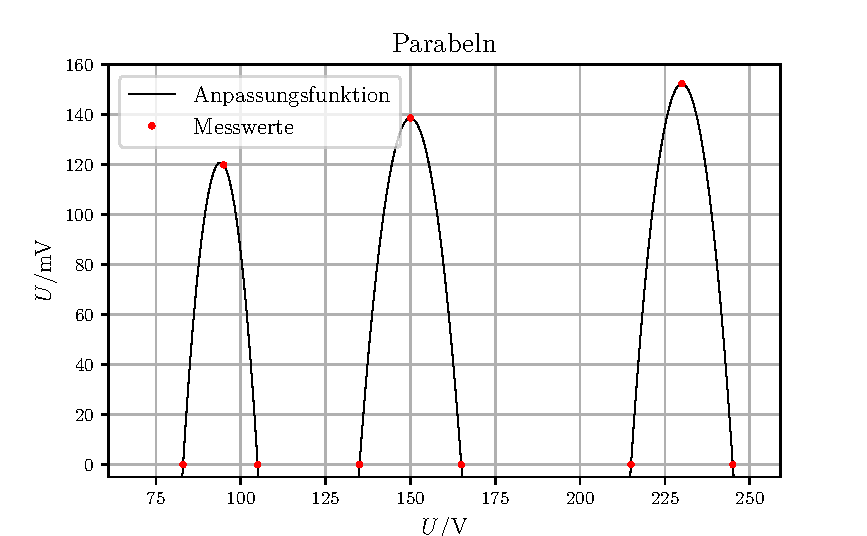
\includegraphics{plot1.pdf}
  \caption{Anpassungsfunktionen für die Messwerte der drei Moden}
  \label{fig:plot}
\end{figure}



\subsection{Frtequenz, Wellenlänge und Dämpfung}
Die Abstände der Minima zu dem jeweilligen nächsten Minima betragen $113.0$mm, $90.0$mm,
$65.0$mm und $42.0$mm.
Für den Mittelwert der Wellenlänge im Hohlleiter ergibt sich $\SI{4.73(13)}{\centi\meter}$.



Die Dämpfung $D$, in Abhängigkeit von der Tiefe $d$ der Mikrometerschraube des Abschwächers, ist in Tabelle 2
dargestellt. Dabei sind einmal die gemessenen Werte der Dämpfung $D_1$, sowie die Dämpfungswerte der
Eichkurve $D_2$ angegeben.


\begin{table}[H]
  \centering
  \caption{Dämpfungen in Abhängigkeit von der Tiefe der Mikrometerschraube}
  \label{tab:Parameter}
  \begin{tabular}{c c c}
    \toprule
    $d$/mm & $D_1/$dB & $D_2/$dB\\
    \midrule
    1.0 &  0  & 2.1    \\
    1.7 &  0.2  & 5.9    \\
    2.0 &  0.6  & 7.9    \\
    2.5 &  2.7  & 11.0    \\
    2.8 &  4.9  & 14.0    \\
    2.9 &  6.0  & 15.0    \\
    3.0 &  6.8  & 16.0    \\
    3.1 &  8.1  & 18.0    \\
    3.2 &  8.9  & 19.0    \\
    3.3 &  10.0 & 20.0    \\
    \bottomrule
  \end{tabular}
\end{table}
